% Options for packages loaded elsewhere
\PassOptionsToPackage{unicode}{hyperref}
\PassOptionsToPackage{hyphens}{url}
%
\documentclass[
]{article}
\usepackage{amsmath,amssymb}
\usepackage{iftex}
\ifPDFTeX
  \usepackage[T1]{fontenc}
  \usepackage[utf8]{inputenc}
  \usepackage{textcomp} % provide euro and other symbols
\else % if luatex or xetex
  \usepackage{unicode-math} % this also loads fontspec
  \defaultfontfeatures{Scale=MatchLowercase}
  \defaultfontfeatures[\rmfamily]{Ligatures=TeX,Scale=1}
\fi
\usepackage{lmodern}
\ifPDFTeX\else
  % xetex/luatex font selection
\fi
% Use upquote if available, for straight quotes in verbatim environments
\IfFileExists{upquote.sty}{\usepackage{upquote}}{}
\IfFileExists{microtype.sty}{% use microtype if available
  \usepackage[]{microtype}
  \UseMicrotypeSet[protrusion]{basicmath} % disable protrusion for tt fonts
}{}
\makeatletter
\@ifundefined{KOMAClassName}{% if non-KOMA class
  \IfFileExists{parskip.sty}{%
    \usepackage{parskip}
  }{% else
    \setlength{\parindent}{0pt}
    \setlength{\parskip}{6pt plus 2pt minus 1pt}}
}{% if KOMA class
  \KOMAoptions{parskip=half}}
\makeatother
\usepackage{xcolor}
\usepackage[margin=1in]{geometry}
\usepackage{color}
\usepackage{fancyvrb}
\newcommand{\VerbBar}{|}
\newcommand{\VERB}{\Verb[commandchars=\\\{\}]}
\DefineVerbatimEnvironment{Highlighting}{Verbatim}{commandchars=\\\{\}}
% Add ',fontsize=\small' for more characters per line
\usepackage{framed}
\definecolor{shadecolor}{RGB}{248,248,248}
\newenvironment{Shaded}{\begin{snugshade}}{\end{snugshade}}
\newcommand{\AlertTok}[1]{\textcolor[rgb]{0.94,0.16,0.16}{#1}}
\newcommand{\AnnotationTok}[1]{\textcolor[rgb]{0.56,0.35,0.01}{\textbf{\textit{#1}}}}
\newcommand{\AttributeTok}[1]{\textcolor[rgb]{0.13,0.29,0.53}{#1}}
\newcommand{\BaseNTok}[1]{\textcolor[rgb]{0.00,0.00,0.81}{#1}}
\newcommand{\BuiltInTok}[1]{#1}
\newcommand{\CharTok}[1]{\textcolor[rgb]{0.31,0.60,0.02}{#1}}
\newcommand{\CommentTok}[1]{\textcolor[rgb]{0.56,0.35,0.01}{\textit{#1}}}
\newcommand{\CommentVarTok}[1]{\textcolor[rgb]{0.56,0.35,0.01}{\textbf{\textit{#1}}}}
\newcommand{\ConstantTok}[1]{\textcolor[rgb]{0.56,0.35,0.01}{#1}}
\newcommand{\ControlFlowTok}[1]{\textcolor[rgb]{0.13,0.29,0.53}{\textbf{#1}}}
\newcommand{\DataTypeTok}[1]{\textcolor[rgb]{0.13,0.29,0.53}{#1}}
\newcommand{\DecValTok}[1]{\textcolor[rgb]{0.00,0.00,0.81}{#1}}
\newcommand{\DocumentationTok}[1]{\textcolor[rgb]{0.56,0.35,0.01}{\textbf{\textit{#1}}}}
\newcommand{\ErrorTok}[1]{\textcolor[rgb]{0.64,0.00,0.00}{\textbf{#1}}}
\newcommand{\ExtensionTok}[1]{#1}
\newcommand{\FloatTok}[1]{\textcolor[rgb]{0.00,0.00,0.81}{#1}}
\newcommand{\FunctionTok}[1]{\textcolor[rgb]{0.13,0.29,0.53}{\textbf{#1}}}
\newcommand{\ImportTok}[1]{#1}
\newcommand{\InformationTok}[1]{\textcolor[rgb]{0.56,0.35,0.01}{\textbf{\textit{#1}}}}
\newcommand{\KeywordTok}[1]{\textcolor[rgb]{0.13,0.29,0.53}{\textbf{#1}}}
\newcommand{\NormalTok}[1]{#1}
\newcommand{\OperatorTok}[1]{\textcolor[rgb]{0.81,0.36,0.00}{\textbf{#1}}}
\newcommand{\OtherTok}[1]{\textcolor[rgb]{0.56,0.35,0.01}{#1}}
\newcommand{\PreprocessorTok}[1]{\textcolor[rgb]{0.56,0.35,0.01}{\textit{#1}}}
\newcommand{\RegionMarkerTok}[1]{#1}
\newcommand{\SpecialCharTok}[1]{\textcolor[rgb]{0.81,0.36,0.00}{\textbf{#1}}}
\newcommand{\SpecialStringTok}[1]{\textcolor[rgb]{0.31,0.60,0.02}{#1}}
\newcommand{\StringTok}[1]{\textcolor[rgb]{0.31,0.60,0.02}{#1}}
\newcommand{\VariableTok}[1]{\textcolor[rgb]{0.00,0.00,0.00}{#1}}
\newcommand{\VerbatimStringTok}[1]{\textcolor[rgb]{0.31,0.60,0.02}{#1}}
\newcommand{\WarningTok}[1]{\textcolor[rgb]{0.56,0.35,0.01}{\textbf{\textit{#1}}}}
\usepackage{longtable,booktabs,array}
\usepackage{calc} % for calculating minipage widths
% Correct order of tables after \paragraph or \subparagraph
\usepackage{etoolbox}
\makeatletter
\patchcmd\longtable{\par}{\if@noskipsec\mbox{}\fi\par}{}{}
\makeatother
% Allow footnotes in longtable head/foot
\IfFileExists{footnotehyper.sty}{\usepackage{footnotehyper}}{\usepackage{footnote}}
\makesavenoteenv{longtable}
\usepackage{graphicx}
\makeatletter
\def\maxwidth{\ifdim\Gin@nat@width>\linewidth\linewidth\else\Gin@nat@width\fi}
\def\maxheight{\ifdim\Gin@nat@height>\textheight\textheight\else\Gin@nat@height\fi}
\makeatother
% Scale images if necessary, so that they will not overflow the page
% margins by default, and it is still possible to overwrite the defaults
% using explicit options in \includegraphics[width, height, ...]{}
\setkeys{Gin}{width=\maxwidth,height=\maxheight,keepaspectratio}
% Set default figure placement to htbp
\makeatletter
\def\fps@figure{htbp}
\makeatother
\setlength{\emergencystretch}{3em} % prevent overfull lines
\providecommand{\tightlist}{%
  \setlength{\itemsep}{0pt}\setlength{\parskip}{0pt}}
\setcounter{secnumdepth}{-\maxdimen} % remove section numbering
\ifLuaTeX
  \usepackage{selnolig}  % disable illegal ligatures
\fi
\usepackage{bookmark}
\IfFileExists{xurl.sty}{\usepackage{xurl}}{} % add URL line breaks if available
\urlstyle{same}
\hypersetup{
  pdftitle={Class 10: Halloween Mini-Project},
  pdfauthor={Diana Furlan},
  hidelinks,
  pdfcreator={LaTeX via pandoc}}

\title{Class 10: Halloween Mini-Project}
\author{Diana Furlan}
\date{2024-10-28}

\begin{document}
\maketitle

\#\#1. Importing candy data

\begin{Shaded}
\begin{Highlighting}[]
\NormalTok{url }\OtherTok{\textless{}{-}} \StringTok{"https://raw.githubusercontent.com/fivethirtyeight/data/master/candy{-}power{-}ranking/candy{-}data.csv"}

\NormalTok{candy\_file }\OtherTok{\textless{}{-}} \FunctionTok{read.csv}\NormalTok{(url)}
\NormalTok{candy }\OtherTok{=} \FunctionTok{read.csv}\NormalTok{(url, }\AttributeTok{row.names=}\DecValTok{1}\NormalTok{)}
\FunctionTok{head}\NormalTok{(candy)}
\end{Highlighting}
\end{Shaded}

\begin{verbatim}
##              chocolate fruity caramel peanutyalmondy nougat crispedricewafer
## 100 Grand            1      0       1              0      0                1
## 3 Musketeers         1      0       0              0      1                0
## One dime             0      0       0              0      0                0
## One quarter          0      0       0              0      0                0
## Air Heads            0      1       0              0      0                0
## Almond Joy           1      0       0              1      0                0
##              hard bar pluribus sugarpercent pricepercent winpercent
## 100 Grand       0   1        0        0.732        0.860   66.97173
## 3 Musketeers    0   1        0        0.604        0.511   67.60294
## One dime        0   0        0        0.011        0.116   32.26109
## One quarter     0   0        0        0.011        0.511   46.11650
## Air Heads       0   0        0        0.906        0.511   52.34146
## Almond Joy      0   1        0        0.465        0.767   50.34755
\end{verbatim}

\#\#What is in the dataset?

\begin{quote}
Q1. How many different candy types are in this dataset?
\end{quote}

\begin{Shaded}
\begin{Highlighting}[]
\NormalTok{candies }\OtherTok{\textless{}{-}} \FunctionTok{nrow}\NormalTok{(candy)}
\NormalTok{candies}
\end{Highlighting}
\end{Shaded}

\begin{verbatim}
## [1] 85
\end{verbatim}

\begin{quote}
Q2. How many fruity candy types are in the dataset?
\end{quote}

\begin{Shaded}
\begin{Highlighting}[]
\NormalTok{fruity }\OtherTok{\textless{}{-}} \FunctionTok{sum}\NormalTok{(candy}\SpecialCharTok{$}\NormalTok{fruity }\SpecialCharTok{==} \DecValTok{1}\NormalTok{)}
\NormalTok{fruity}
\end{Highlighting}
\end{Shaded}

\begin{verbatim}
## [1] 38
\end{verbatim}

\#\#What is your favorate candy?

\begin{quote}
Q3. What is your favorite candy in the dataset and what is it's
winpercent value?
\end{quote}

\begin{Shaded}
\begin{Highlighting}[]
\NormalTok{candy[}\StringTok{"Almond Joy"}\NormalTok{, ]}\SpecialCharTok{$}\NormalTok{winpercent}
\end{Highlighting}
\end{Shaded}

\begin{verbatim}
## [1] 50.34755
\end{verbatim}

\begin{quote}
Q4. What is the winpercent value for ``Kit Kat''?
\end{quote}

\begin{Shaded}
\begin{Highlighting}[]
\NormalTok{candy[}\StringTok{"Kit Kat"}\NormalTok{, ]}\SpecialCharTok{$}\NormalTok{winpercent}
\end{Highlighting}
\end{Shaded}

\begin{verbatim}
## [1] 76.7686
\end{verbatim}

\begin{quote}
Q5. What is the winpercent value for ``Tootsie Roll Snack Bars''?
\end{quote}

\begin{Shaded}
\begin{Highlighting}[]
\NormalTok{candy[}\StringTok{"Tootsie Roll Snack Bars"}\NormalTok{, ]}\SpecialCharTok{$}\NormalTok{winpercent}
\end{Highlighting}
\end{Shaded}

\begin{verbatim}
## [1] 49.6535
\end{verbatim}

There is a useful'skim()'function in the skimr package that can help
give you a quick overview of a given dataset

\begin{Shaded}
\begin{Highlighting}[]
\CommentTok{\#install.packages("skimr")}
\FunctionTok{library}\NormalTok{(}\StringTok{"skimr"}\NormalTok{)}
\CommentTok{\#or just extract a part from the library }
\CommentTok{\#skimr::skim(candy)}
\FunctionTok{skim}\NormalTok{(candy)}
\end{Highlighting}
\end{Shaded}

\begin{longtable}[]{@{}ll@{}}
\caption{Data summary}\tabularnewline
\toprule\noalign{}
\endfirsthead
\endhead
\bottomrule\noalign{}
\endlastfoot
Name & candy \\
Number of rows & 85 \\
Number of columns & 12 \\
\_\_\_\_\_\_\_\_\_\_\_\_\_\_\_\_\_\_\_\_\_\_\_ & \\
Column type frequency: & \\
numeric & 12 \\
\_\_\_\_\_\_\_\_\_\_\_\_\_\_\_\_\_\_\_\_\_\_\_\_ & \\
Group variables & None \\
\end{longtable}

\textbf{Variable type: numeric}

\begin{longtable}[]{@{}
  >{\raggedright\arraybackslash}p{(\columnwidth - 20\tabcolsep) * \real{0.1910}}
  >{\raggedleft\arraybackslash}p{(\columnwidth - 20\tabcolsep) * \real{0.1124}}
  >{\raggedleft\arraybackslash}p{(\columnwidth - 20\tabcolsep) * \real{0.1573}}
  >{\raggedleft\arraybackslash}p{(\columnwidth - 20\tabcolsep) * \real{0.0674}}
  >{\raggedleft\arraybackslash}p{(\columnwidth - 20\tabcolsep) * \real{0.0674}}
  >{\raggedleft\arraybackslash}p{(\columnwidth - 20\tabcolsep) * \real{0.0674}}
  >{\raggedleft\arraybackslash}p{(\columnwidth - 20\tabcolsep) * \real{0.0674}}
  >{\raggedleft\arraybackslash}p{(\columnwidth - 20\tabcolsep) * \real{0.0674}}
  >{\raggedleft\arraybackslash}p{(\columnwidth - 20\tabcolsep) * \real{0.0674}}
  >{\raggedleft\arraybackslash}p{(\columnwidth - 20\tabcolsep) * \real{0.0674}}
  >{\raggedright\arraybackslash}p{(\columnwidth - 20\tabcolsep) * \real{0.0674}}@{}}
\toprule\noalign{}
\begin{minipage}[b]{\linewidth}\raggedright
skim\_variable
\end{minipage} & \begin{minipage}[b]{\linewidth}\raggedleft
n\_missing
\end{minipage} & \begin{minipage}[b]{\linewidth}\raggedleft
complete\_rate
\end{minipage} & \begin{minipage}[b]{\linewidth}\raggedleft
mean
\end{minipage} & \begin{minipage}[b]{\linewidth}\raggedleft
sd
\end{minipage} & \begin{minipage}[b]{\linewidth}\raggedleft
p0
\end{minipage} & \begin{minipage}[b]{\linewidth}\raggedleft
p25
\end{minipage} & \begin{minipage}[b]{\linewidth}\raggedleft
p50
\end{minipage} & \begin{minipage}[b]{\linewidth}\raggedleft
p75
\end{minipage} & \begin{minipage}[b]{\linewidth}\raggedleft
p100
\end{minipage} & \begin{minipage}[b]{\linewidth}\raggedright
hist
\end{minipage} \\
\midrule\noalign{}
\endhead
\bottomrule\noalign{}
\endlastfoot
chocolate & 0 & 1 & 0.44 & 0.50 & 0.00 & 0.00 & 0.00 & 1.00 & 1.00 &
▇▁▁▁▆ \\
fruity & 0 & 1 & 0.45 & 0.50 & 0.00 & 0.00 & 0.00 & 1.00 & 1.00 &
▇▁▁▁▆ \\
caramel & 0 & 1 & 0.16 & 0.37 & 0.00 & 0.00 & 0.00 & 0.00 & 1.00 &
▇▁▁▁▂ \\
peanutyalmondy & 0 & 1 & 0.16 & 0.37 & 0.00 & 0.00 & 0.00 & 0.00 & 1.00
& ▇▁▁▁▂ \\
nougat & 0 & 1 & 0.08 & 0.28 & 0.00 & 0.00 & 0.00 & 0.00 & 1.00 &
▇▁▁▁▁ \\
crispedricewafer & 0 & 1 & 0.08 & 0.28 & 0.00 & 0.00 & 0.00 & 0.00 &
1.00 & ▇▁▁▁▁ \\
hard & 0 & 1 & 0.18 & 0.38 & 0.00 & 0.00 & 0.00 & 0.00 & 1.00 & ▇▁▁▁▂ \\
bar & 0 & 1 & 0.25 & 0.43 & 0.00 & 0.00 & 0.00 & 0.00 & 1.00 & ▇▁▁▁▂ \\
pluribus & 0 & 1 & 0.52 & 0.50 & 0.00 & 0.00 & 1.00 & 1.00 & 1.00 &
▇▁▁▁▇ \\
sugarpercent & 0 & 1 & 0.48 & 0.28 & 0.01 & 0.22 & 0.47 & 0.73 & 0.99 &
▇▇▇▇▆ \\
pricepercent & 0 & 1 & 0.47 & 0.29 & 0.01 & 0.26 & 0.47 & 0.65 & 0.98 &
▇▇▇▇▆ \\
winpercent & 0 & 1 & 50.32 & 14.71 & 22.45 & 39.14 & 47.83 & 59.86 &
84.18 & ▃▇▆▅▂ \\
\end{longtable}

we have to scale the winpercent

\begin{quote}
Q6. Is there any variable/column that looks to be on a different scale
to the majority of the other columns in the dataset? sugarpercent,
pricepercent and winpercent are on a non binary scale.
\end{quote}

\begin{quote}
Q7. What do you think a zero and one represent for the candy\$chocolate
column? 1 = T for chocolate and 0 = F for chocolate
\end{quote}

\begin{center}\rule{0.5\linewidth}{0.5pt}\end{center}

\begin{quote}
Q8. Plot a histogram of winpercent values
\end{quote}

\begin{Shaded}
\begin{Highlighting}[]
\CommentTok{\#can add color with \textquotesingle{}col\textquotesingle{}{-} how to change the title?}

\FunctionTok{hist}\NormalTok{(candy}\SpecialCharTok{$}\NormalTok{winpercent, }\AttributeTok{xlab =} \StringTok{"Win Percent"}\NormalTok{)}
  \FunctionTok{abline}\NormalTok{(}\AttributeTok{v =} \DecValTok{50}\NormalTok{, }\AttributeTok{col =} \StringTok{"red"}\NormalTok{)}
\end{Highlighting}
\end{Shaded}

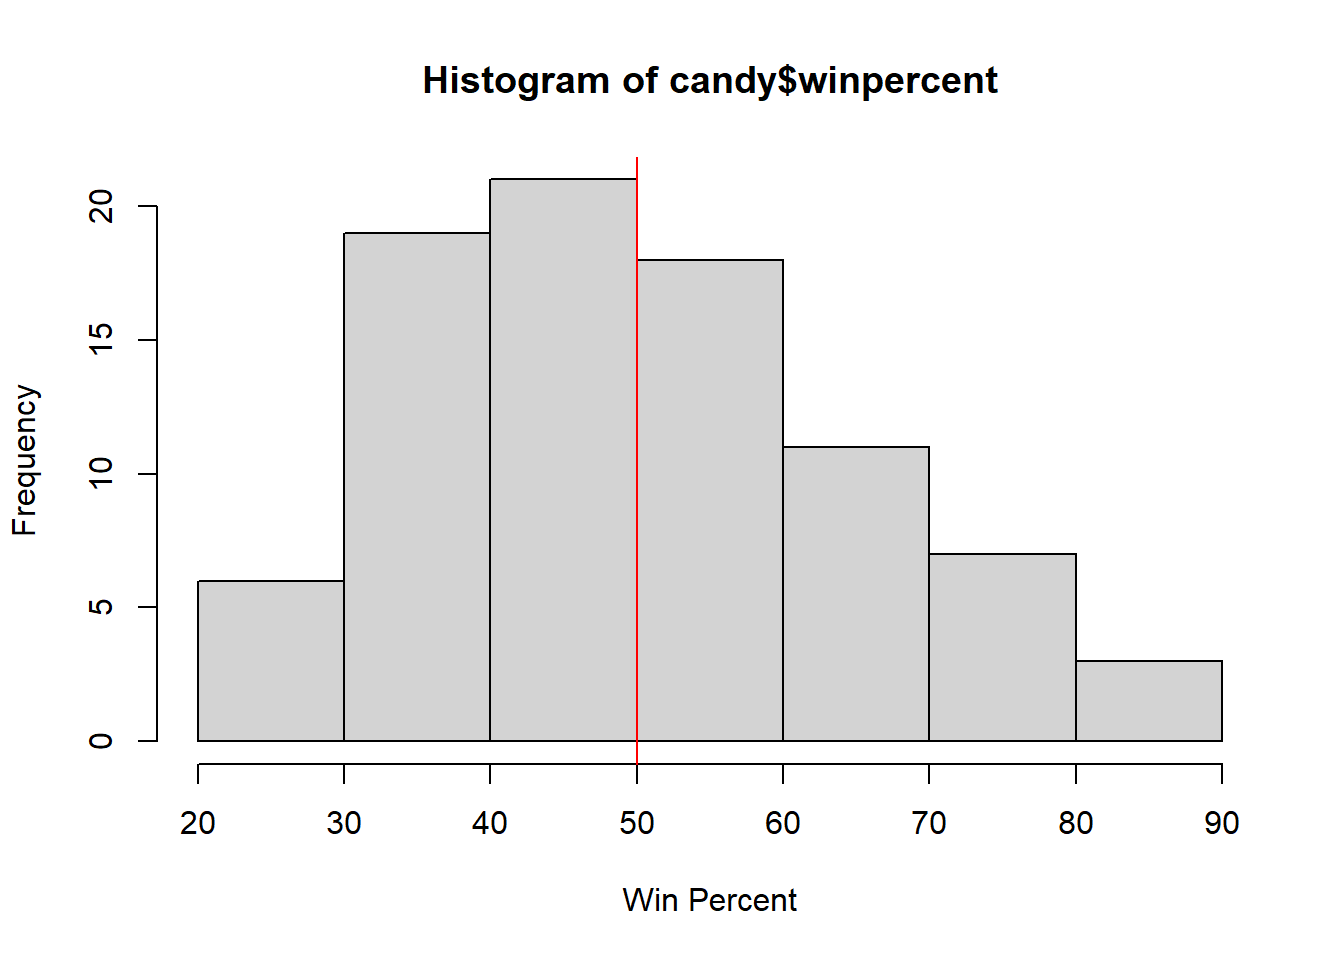
\includegraphics{Halloween-Candy-Mini-Project_files/figure-latex/unnamed-chunk-8-1.pdf}

\begin{Shaded}
\begin{Highlighting}[]
\FunctionTok{library}\NormalTok{(ggplot2)}

\FunctionTok{ggplot}\NormalTok{(candy) }\SpecialCharTok{+}
  \FunctionTok{aes}\NormalTok{(winpercent) }\SpecialCharTok{+}
  \FunctionTok{geom\_histogram}\NormalTok{(}\AttributeTok{binwidth =} \DecValTok{8}\NormalTok{) }
\end{Highlighting}
\end{Shaded}

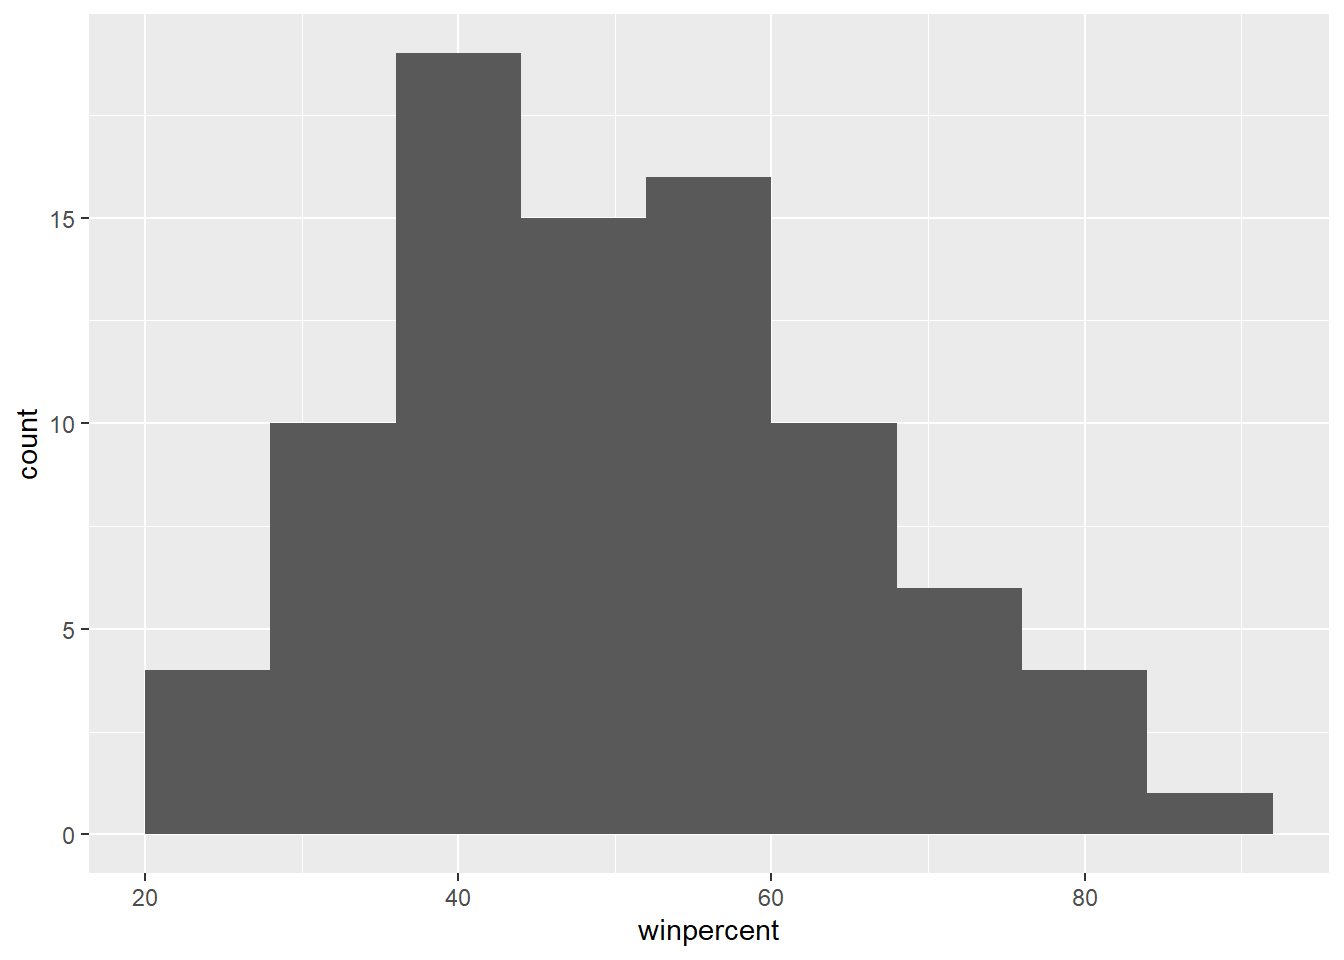
\includegraphics{Halloween-Candy-Mini-Project_files/figure-latex/unnamed-chunk-9-1.pdf}

\begin{quote}
Q9. Is the distribution of winpercent values symmetrical? slighly
right-skewed
\end{quote}

\begin{quote}
Q10. Is the center of the distribution above or below 50\%? slightly
above 50\%
\end{quote}

\begin{Shaded}
\begin{Highlighting}[]
\FunctionTok{summary}\NormalTok{(candy}\SpecialCharTok{$}\NormalTok{winpercent)}
\end{Highlighting}
\end{Shaded}

\begin{verbatim}
##    Min. 1st Qu.  Median    Mean 3rd Qu.    Max. 
##   22.45   39.14   47.83   50.32   59.86   84.18
\end{verbatim}

\begin{quote}
Q11. On average is chocolate candy higher or lower ranked than fruit
candy? chocolate seems higher
\end{quote}

\begin{Shaded}
\begin{Highlighting}[]
\FunctionTok{summary}\NormalTok{(candy[}\FunctionTok{as.logical}\NormalTok{(candy}\SpecialCharTok{$}\NormalTok{chocolate),]}\SpecialCharTok{$}\NormalTok{winpercent)}
\end{Highlighting}
\end{Shaded}

\begin{verbatim}
##    Min. 1st Qu.  Median    Mean 3rd Qu.    Max. 
##   34.72   50.35   60.80   60.92   70.74   84.18
\end{verbatim}

\begin{Shaded}
\begin{Highlighting}[]
\CommentTok{\#installed.packages("dplyr")}
\end{Highlighting}
\end{Shaded}

\begin{Shaded}
\begin{Highlighting}[]
\FunctionTok{library}\NormalTok{(dplyr)}
\end{Highlighting}
\end{Shaded}

\begin{verbatim}
## 
## Attaching package: 'dplyr'
\end{verbatim}

\begin{verbatim}
## The following objects are masked from 'package:stats':
## 
##     filter, lag
\end{verbatim}

\begin{verbatim}
## The following objects are masked from 'package:base':
## 
##     intersect, setdiff, setequal, union
\end{verbatim}

\begin{Shaded}
\begin{Highlighting}[]
\NormalTok{fruit.candy }\OtherTok{\textless{}{-}}\NormalTok{ candy }\SpecialCharTok{|\textgreater{}}
   \FunctionTok{filter}\NormalTok{(fruity}\SpecialCharTok{==}\DecValTok{1}\NormalTok{)}

\FunctionTok{summary}\NormalTok{(fruit.candy}\SpecialCharTok{$}\NormalTok{winpercent)}
\end{Highlighting}
\end{Shaded}

\begin{verbatim}
##    Min. 1st Qu.  Median    Mean 3rd Qu.    Max. 
##   22.45   39.04   42.97   44.12   52.11   67.04
\end{verbatim}

\begin{quote}
Q12. Is this difference statistically significant?
\end{quote}

\begin{Shaded}
\begin{Highlighting}[]
\NormalTok{choc.candy }\OtherTok{\textless{}{-}}\NormalTok{ candy }\SpecialCharTok{|\textgreater{}} \FunctionTok{filter}\NormalTok{(chocolate }\SpecialCharTok{==}\DecValTok{1}\NormalTok{)}
\NormalTok{fruit.candy }\OtherTok{\textless{}{-}}\NormalTok{ candy }\SpecialCharTok{|\textgreater{}} \FunctionTok{filter}\NormalTok{(fruity }\SpecialCharTok{==} \DecValTok{1}\NormalTok{)}
\end{Highlighting}
\end{Shaded}

\begin{Shaded}
\begin{Highlighting}[]
\NormalTok{t\_test\_result }\OtherTok{\textless{}{-}} \FunctionTok{t.test}\NormalTok{(choc.candy}\SpecialCharTok{$}\NormalTok{winpercent, fruit.candy}\SpecialCharTok{$}\NormalTok{winpercent)}

\NormalTok{t\_test\_result}
\end{Highlighting}
\end{Shaded}

\begin{verbatim}
## 
##  Welch Two Sample t-test
## 
## data:  choc.candy$winpercent and fruit.candy$winpercent
## t = 6.2582, df = 68.882, p-value = 2.871e-08
## alternative hypothesis: true difference in means is not equal to 0
## 95 percent confidence interval:
##  11.44563 22.15795
## sample estimates:
## mean of x mean of y 
##  60.92153  44.11974
\end{verbatim}

\#\#Overall Candy Rankings

\begin{Shaded}
\begin{Highlighting}[]
\NormalTok{play }\OtherTok{\textless{}{-}} \FunctionTok{c}\NormalTok{(}\StringTok{"d"}\NormalTok{,}\StringTok{"a"}\NormalTok{,}\StringTok{"c"}\NormalTok{)}
\FunctionTok{sort}\NormalTok{(play)}
\end{Highlighting}
\end{Shaded}

\begin{verbatim}
## [1] "a" "c" "d"
\end{verbatim}

\begin{Shaded}
\begin{Highlighting}[]
\FunctionTok{order}\NormalTok{(play)}
\end{Highlighting}
\end{Shaded}

\begin{verbatim}
## [1] 2 3 1
\end{verbatim}

\begin{Shaded}
\begin{Highlighting}[]
\NormalTok{play[}\FunctionTok{order}\NormalTok{(play) ]}
\end{Highlighting}
\end{Shaded}

\begin{verbatim}
## [1] "a" "c" "d"
\end{verbatim}

\begin{quote}
Q13. What are the five least liked candy types in this set?
\end{quote}

\begin{Shaded}
\begin{Highlighting}[]
\FunctionTok{sort}\NormalTok{(}\FunctionTok{c}\NormalTok{(}\DecValTok{5}\NormalTok{, }\DecValTok{2}\NormalTok{, }\DecValTok{10}\NormalTok{), }\AttributeTok{decreasing =}\NormalTok{ T)}
\end{Highlighting}
\end{Shaded}

\begin{verbatim}
## [1] 10  5  2
\end{verbatim}

\begin{Shaded}
\begin{Highlighting}[]
\FunctionTok{head}\NormalTok{( candy[}\FunctionTok{order}\NormalTok{(candy}\SpecialCharTok{$}\NormalTok{winpercent),], }\DecValTok{5}\NormalTok{)}
\end{Highlighting}
\end{Shaded}

\begin{verbatim}
##                    chocolate fruity caramel peanutyalmondy nougat
## Nik L Nip                  0      1       0              0      0
## Boston Baked Beans         0      0       0              1      0
## Chiclets                   0      1       0              0      0
## Super Bubble               0      1       0              0      0
## Jawbusters                 0      1       0              0      0
##                    crispedricewafer hard bar pluribus sugarpercent pricepercent
## Nik L Nip                         0    0   0        1        0.197        0.976
## Boston Baked Beans                0    0   0        1        0.313        0.511
## Chiclets                          0    0   0        1        0.046        0.325
## Super Bubble                      0    0   0        0        0.162        0.116
## Jawbusters                        0    1   0        1        0.093        0.511
##                    winpercent
## Nik L Nip            22.44534
## Boston Baked Beans   23.41782
## Chiclets             24.52499
## Super Bubble         27.30386
## Jawbusters           28.12744
\end{verbatim}

\begin{quote}
Q14. What are the top 5 all time favorite candy types out of this set?
\end{quote}

\begin{Shaded}
\begin{Highlighting}[]
\NormalTok{candy}\SpecialCharTok{\%\textgreater{}\%}
  \FunctionTok{arrange}\NormalTok{(winpercent) }\SpecialCharTok{\%\textgreater{}\%} \FunctionTok{head}\NormalTok{(}\DecValTok{5}\NormalTok{)}
\end{Highlighting}
\end{Shaded}

\begin{verbatim}
##                    chocolate fruity caramel peanutyalmondy nougat
## Nik L Nip                  0      1       0              0      0
## Boston Baked Beans         0      0       0              1      0
## Chiclets                   0      1       0              0      0
## Super Bubble               0      1       0              0      0
## Jawbusters                 0      1       0              0      0
##                    crispedricewafer hard bar pluribus sugarpercent pricepercent
## Nik L Nip                         0    0   0        1        0.197        0.976
## Boston Baked Beans                0    0   0        1        0.313        0.511
## Chiclets                          0    0   0        1        0.046        0.325
## Super Bubble                      0    0   0        0        0.162        0.116
## Jawbusters                        0    1   0        1        0.093        0.511
##                    winpercent
## Nik L Nip            22.44534
## Boston Baked Beans   23.41782
## Chiclets             24.52499
## Super Bubble         27.30386
## Jawbusters           28.12744
\end{verbatim}

\begin{quote}
Q15. Make a first barplot of candy ranking based on winpercent values.
\end{quote}

Bar plot

\begin{Shaded}
\begin{Highlighting}[]
\FunctionTok{library}\NormalTok{(ggplot2)}

\FunctionTok{ggplot}\NormalTok{(candy) }\SpecialCharTok{+}
  \FunctionTok{aes}\NormalTok{(winpercent, }\FunctionTok{rownames}\NormalTok{(candy)) }\SpecialCharTok{+}
  \FunctionTok{geom\_col}\NormalTok{()}
\end{Highlighting}
\end{Shaded}

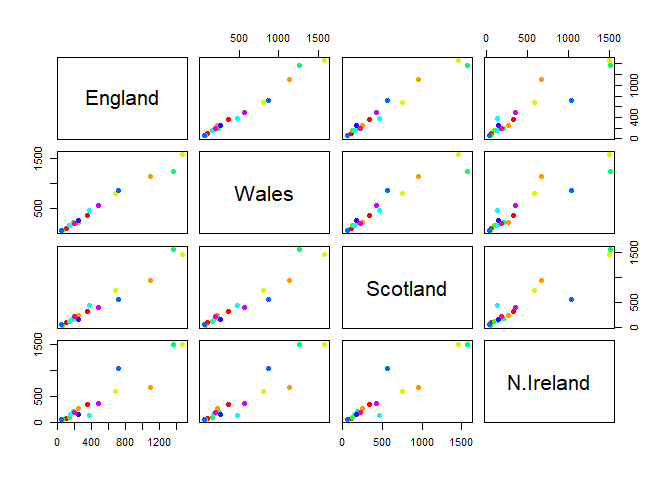
\includegraphics{Halloween-Candy-Mini-Project_files/figure-latex/unnamed-chunk-21-1.pdf}

\begin{quote}
Q16. This is quite ugly, use the reorder() function to get the bars
sorted by winpercent?
\end{quote}

Bar plot

\begin{Shaded}
\begin{Highlighting}[]
\FunctionTok{ggplot}\NormalTok{(candy) }\SpecialCharTok{+}
  \FunctionTok{aes}\NormalTok{(}\AttributeTok{x=}\NormalTok{winpercent, }
      \AttributeTok{y=}\FunctionTok{reorder}\NormalTok{(}\FunctionTok{rownames}\NormalTok{(candy), winpercent),}
      \AttributeTok{fill=}\NormalTok{ chocolate) }\SpecialCharTok{+}
  \FunctionTok{geom\_col}\NormalTok{()}
\end{Highlighting}
\end{Shaded}

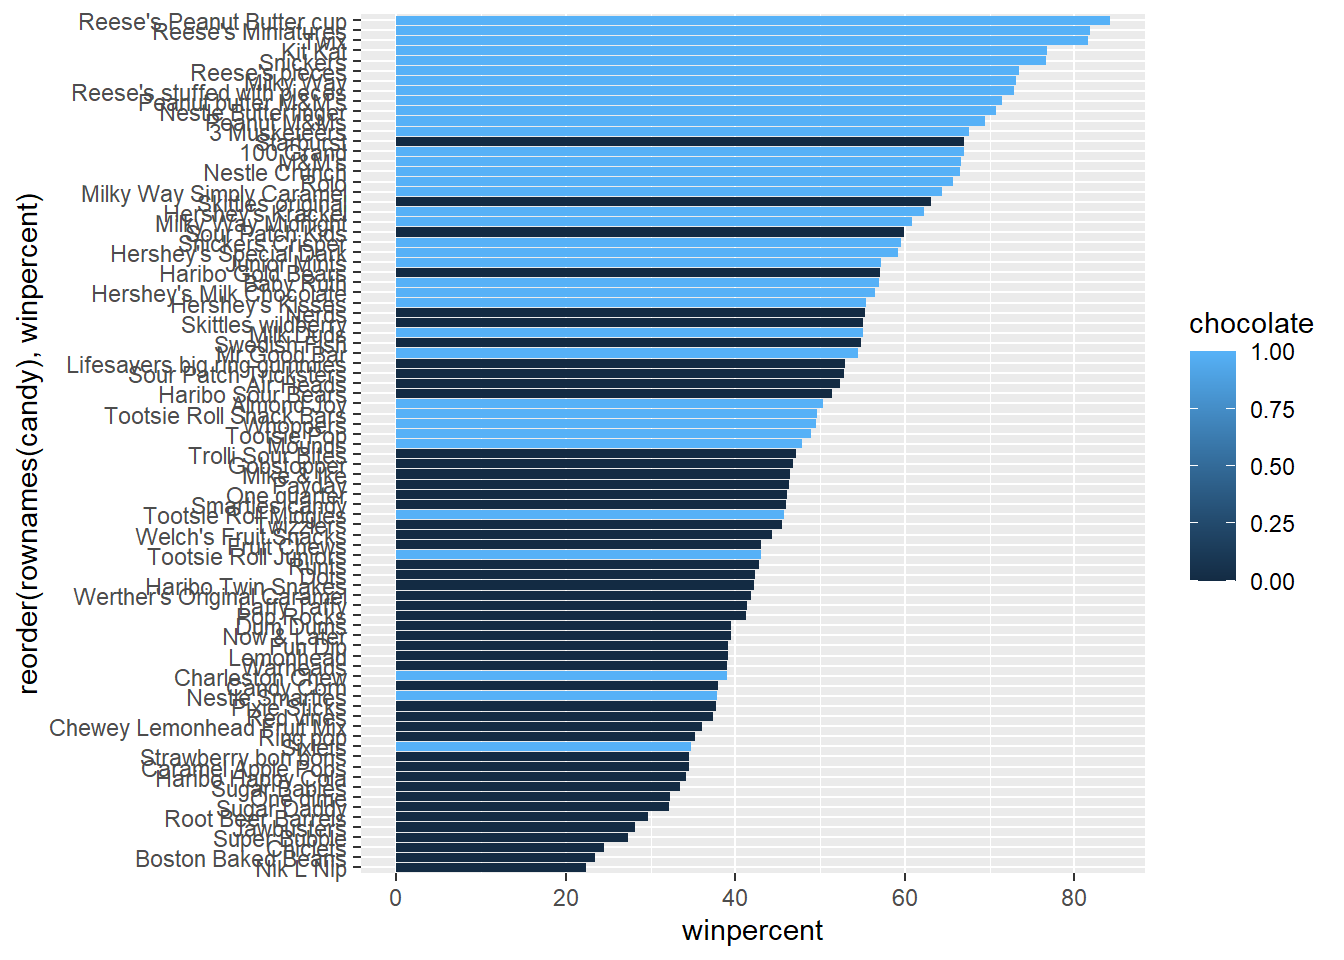
\includegraphics{Halloween-Candy-Mini-Project_files/figure-latex/unnamed-chunk-22-1.pdf}

More custom col skim so we can see both chocolate and bar and fruity,
etc. all from the same plot

\begin{Shaded}
\begin{Highlighting}[]
\NormalTok{mycols }\OtherTok{\textless{}{-}} \FunctionTok{rep}\NormalTok{(}\StringTok{"black"}\NormalTok{, }\FunctionTok{nrow}\NormalTok{(candy))}
\NormalTok{mycols[}\FunctionTok{as.logical}\NormalTok{(candy}\SpecialCharTok{$}\NormalTok{chocolate)] }\OtherTok{\textless{}{-}} \StringTok{"chocolate"}
\NormalTok{mycols [}\FunctionTok{as.logical}\NormalTok{(candy}\SpecialCharTok{$}\NormalTok{bar)] }\OtherTok{\textless{}{-}} \StringTok{"brown"}
\NormalTok{mycols [}\FunctionTok{as.logical}\NormalTok{(candy}\SpecialCharTok{$}\NormalTok{fruity)] }\OtherTok{\textless{}{-}} \StringTok{"pink"}
\CommentTok{\#use blue for my fav candy}
\end{Highlighting}
\end{Shaded}

\begin{Shaded}
\begin{Highlighting}[]
\NormalTok{mycols [}\FunctionTok{rownames}\NormalTok{(candy)}\SpecialCharTok{==}\StringTok{"Almond Joy"}\NormalTok{] }\OtherTok{\textless{}{-}} \StringTok{"blue"}
\NormalTok{mycols}
\end{Highlighting}
\end{Shaded}

\begin{verbatim}
##  [1] "brown"     "brown"     "black"     "black"     "pink"      "blue"     
##  [7] "brown"     "black"     "black"     "pink"      "brown"     "pink"     
## [13] "pink"      "pink"      "pink"      "pink"      "pink"      "pink"     
## [19] "pink"      "black"     "pink"      "pink"      "chocolate" "brown"    
## [25] "brown"     "brown"     "pink"      "chocolate" "brown"     "pink"     
## [31] "pink"      "pink"      "chocolate" "chocolate" "pink"      "chocolate"
## [37] "brown"     "brown"     "brown"     "brown"     "brown"     "pink"     
## [43] "brown"     "brown"     "pink"      "pink"      "brown"     "chocolate"
## [49] "black"     "pink"      "pink"      "chocolate" "chocolate" "chocolate"
## [55] "chocolate" "pink"      "chocolate" "black"     "pink"      "chocolate"
## [61] "pink"      "pink"      "chocolate" "pink"      "brown"     "brown"    
## [67] "pink"      "pink"      "pink"      "pink"      "black"     "black"    
## [73] "pink"      "pink"      "pink"      "chocolate" "chocolate" "brown"    
## [79] "pink"      "brown"     "pink"      "pink"      "pink"      "black"    
## [85] "chocolate"
\end{verbatim}

\begin{Shaded}
\begin{Highlighting}[]
\CommentTok{\#placeholder}
\FunctionTok{ggplot}\NormalTok{(candy) }\SpecialCharTok{+}
  \FunctionTok{aes}\NormalTok{(}\AttributeTok{x=}\NormalTok{winpercent, }
      \AttributeTok{y=}\FunctionTok{reorder}\NormalTok{(}\FunctionTok{rownames}\NormalTok{(candy), winpercent),) }\SpecialCharTok{+}
  \FunctionTok{geom\_col}\NormalTok{(}\AttributeTok{fill =}\NormalTok{mycols)}
\end{Highlighting}
\end{Shaded}

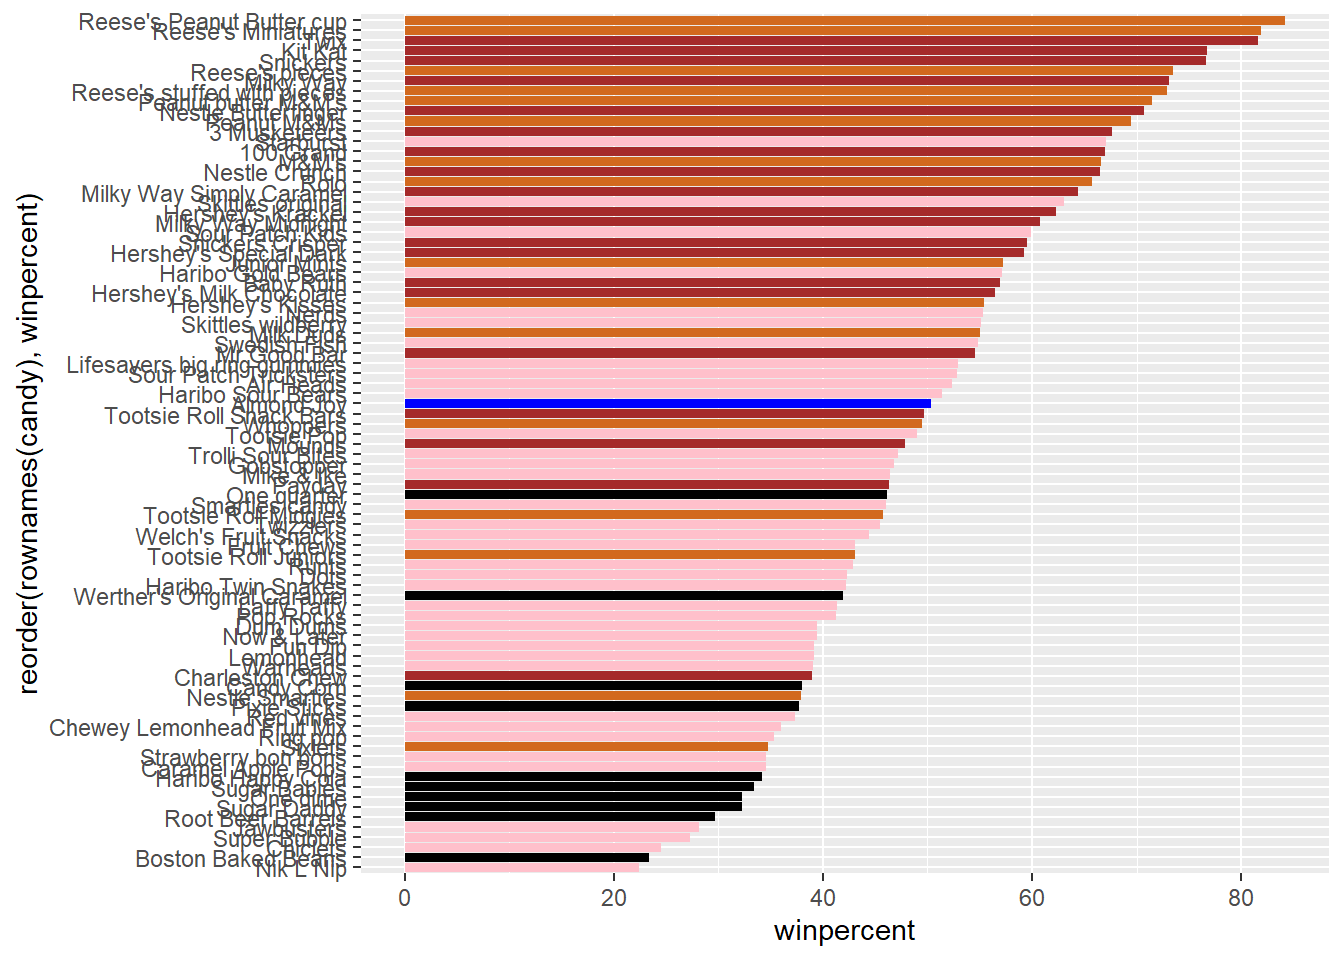
\includegraphics{Halloween-Candy-Mini-Project_files/figure-latex/unnamed-chunk-25-1.pdf}
\textgreater Q17. What is the worst ranked chocolate candy? Nik L Nip

\begin{quote}
Q18. What is the best ranked fruity candy? Starbust
\end{quote}

Plot of win vs Price

\begin{Shaded}
\begin{Highlighting}[]
\NormalTok{mycols[}\FunctionTok{as.logical}\NormalTok{(candy}\SpecialCharTok{$}\NormalTok{fruity)]}\OtherTok{\textless{}{-}} \StringTok{"red"}
\NormalTok{mycols}
\end{Highlighting}
\end{Shaded}

\begin{verbatim}
##  [1] "brown"     "brown"     "black"     "black"     "red"       "blue"     
##  [7] "brown"     "black"     "black"     "red"       "brown"     "red"      
## [13] "red"       "red"       "red"       "red"       "red"       "red"      
## [19] "red"       "black"     "red"       "red"       "chocolate" "brown"    
## [25] "brown"     "brown"     "red"       "chocolate" "brown"     "red"      
## [31] "red"       "red"       "chocolate" "chocolate" "red"       "chocolate"
## [37] "brown"     "brown"     "brown"     "brown"     "brown"     "red"      
## [43] "brown"     "brown"     "red"       "red"       "brown"     "chocolate"
## [49] "black"     "red"       "red"       "chocolate" "chocolate" "chocolate"
## [55] "chocolate" "red"       "chocolate" "black"     "red"       "chocolate"
## [61] "red"       "red"       "chocolate" "red"       "brown"     "brown"    
## [67] "red"       "red"       "red"       "red"       "black"     "black"    
## [73] "red"       "red"       "red"       "chocolate" "chocolate" "brown"    
## [79] "red"       "brown"     "red"       "red"       "red"       "black"    
## [85] "chocolate"
\end{verbatim}

\#\#Taking a look at pricepercent

add labels

\begin{Shaded}
\begin{Highlighting}[]
\CommentTok{\#install.packages("ggrepel")}
\end{Highlighting}
\end{Shaded}

\#\texttt{\{r\}\ library(ggrepel)\ ggplot\ (candy)\ +\ \ \ aes(winpercent,pricepercent,\ label=rownames(candy))\ +\ \ \ geom\_point(col=mycols)\ +\ \ \ geom\_label(col=mycols)\ +\ \ \ geom\_text\_repel(max.overlaps\ =\ 8,\ col=mycols,\ )\ \ \#}

\begin{quote}
Q19. Which candy type is the highest ranked in terms of winpercent for
the least money - i.e.~offers the most bang for your buck?
\end{quote}

\begin{Shaded}
\begin{Highlighting}[]
\FunctionTok{ggplot}\NormalTok{ (candy)}\SpecialCharTok{+}
  \FunctionTok{aes}\NormalTok{(winpercent,pricepercent)}\SpecialCharTok{+}
  \FunctionTok{geom\_point}\NormalTok{(}\AttributeTok{col=}\NormalTok{mycols)}
\end{Highlighting}
\end{Shaded}

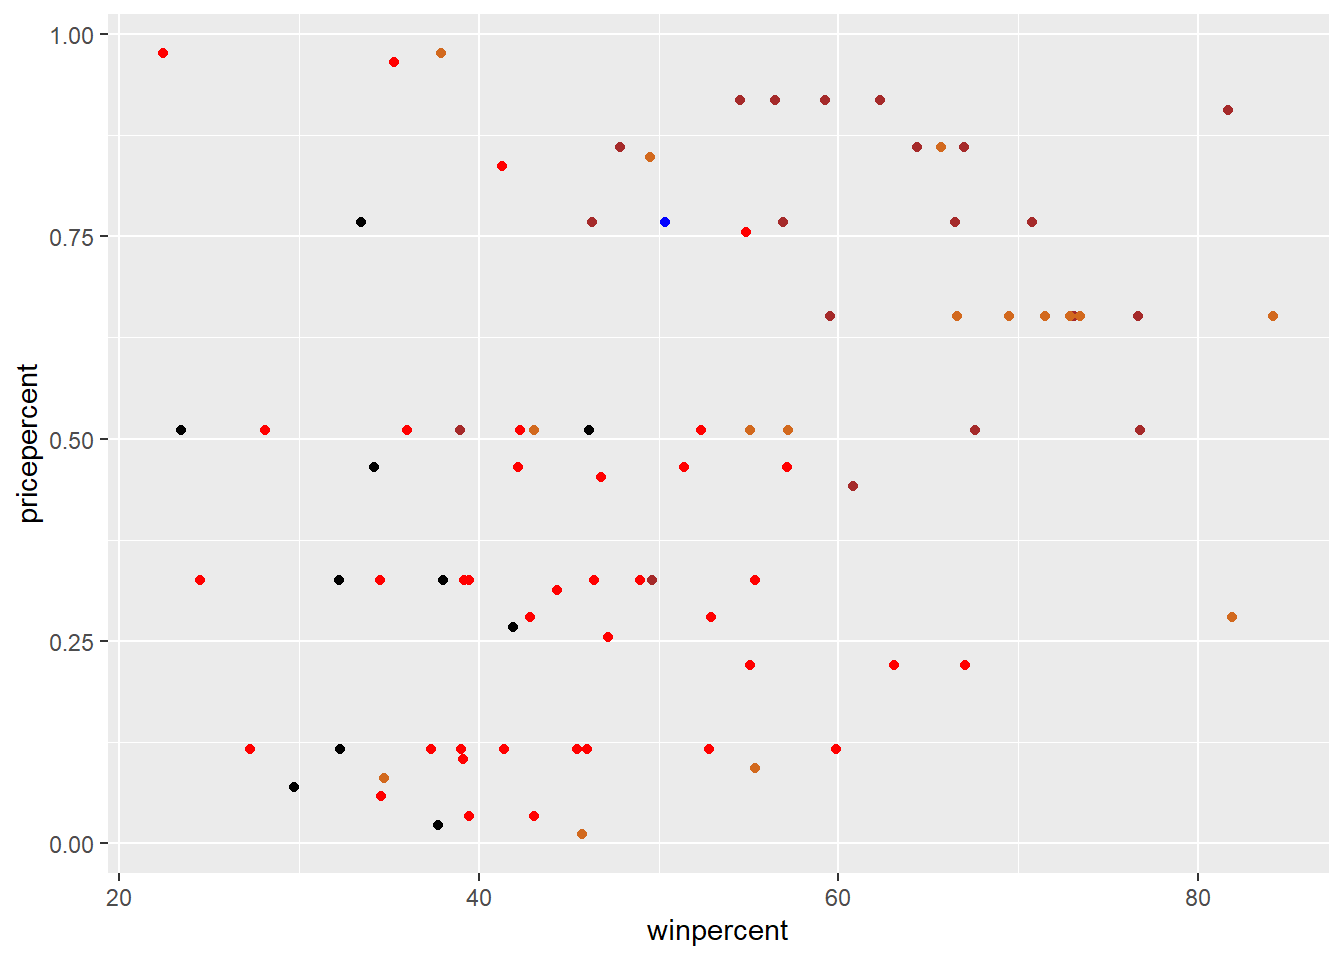
\includegraphics{Halloween-Candy-Mini-Project_files/figure-latex/unnamed-chunk-28-1.pdf}

\begin{quote}
Q20. What are the top 5 most expensive candy types in the dataset and of
these which is the least popular?
\end{quote}

\begin{Shaded}
\begin{Highlighting}[]
\NormalTok{ord }\OtherTok{\textless{}{-}} \FunctionTok{order}\NormalTok{(candy}\SpecialCharTok{$}\NormalTok{pricepercent, }\AttributeTok{decreasing =} \ConstantTok{TRUE}\NormalTok{)}
\FunctionTok{head}\NormalTok{ ( candy[ ord, }\FunctionTok{c}\NormalTok{(}\DecValTok{11}\NormalTok{,}\DecValTok{12}\NormalTok{)], }\AttributeTok{n=}\DecValTok{5}\NormalTok{ )}
\end{Highlighting}
\end{Shaded}

\begin{verbatim}
##                          pricepercent winpercent
## Nik L Nip                       0.976   22.44534
## Nestle Smarties                 0.976   37.88719
## Ring pop                        0.965   35.29076
## Hershey's Krackel               0.918   62.28448
## Hershey's Milk Chocolate        0.918   56.49050
\end{verbatim}

\begin{Shaded}
\begin{Highlighting}[]
\CommentTok{\#install.packages("corrplot")}
\end{Highlighting}
\end{Shaded}

\begin{Shaded}
\begin{Highlighting}[]
\FunctionTok{library}\NormalTok{(corrplot)}
\end{Highlighting}
\end{Shaded}

\begin{verbatim}
## corrplot 0.95 loaded
\end{verbatim}

\begin{Shaded}
\begin{Highlighting}[]
\NormalTok{cij }\OtherTok{\textless{}{-}} \FunctionTok{cor}\NormalTok{(candy)}
\FunctionTok{corrplot}\NormalTok{ (cij, }\AttributeTok{diag=}\NormalTok{F)}
\end{Highlighting}
\end{Shaded}

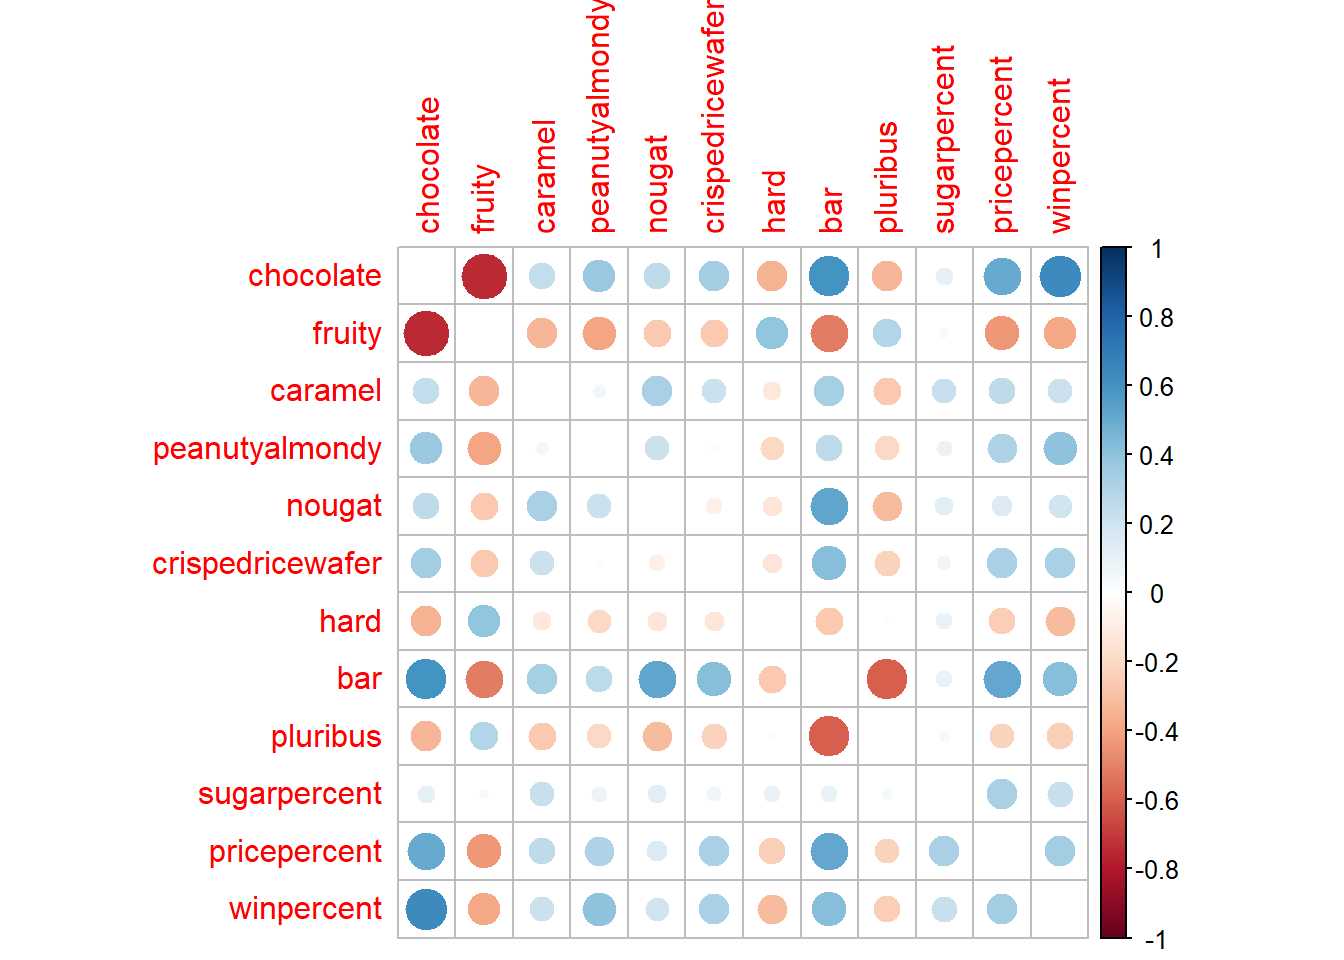
\includegraphics{Halloween-Candy-Mini-Project_files/figure-latex/unnamed-chunk-31-1.pdf}
\textgreater Q22. Examining this plot what two variables are
anti-correlated (i.e.~have minus values)? chocolate and gruit

\begin{quote}
Q23. Similarly, what two variables are most positively correlated?
chocolate and bar
\end{quote}

\#\#Principal Component Analysis

\begin{Shaded}
\begin{Highlighting}[]
\NormalTok{pca }\OtherTok{\textless{}{-}} \FunctionTok{prcomp}\NormalTok{(candy, }\AttributeTok{scale=}\NormalTok{ T)}
\FunctionTok{summary}\NormalTok{(pca)}
\end{Highlighting}
\end{Shaded}

\begin{verbatim}
## Importance of components:
##                           PC1    PC2    PC3     PC4    PC5     PC6     PC7
## Standard deviation     2.0788 1.1378 1.1092 1.07533 0.9518 0.81923 0.81530
## Proportion of Variance 0.3601 0.1079 0.1025 0.09636 0.0755 0.05593 0.05539
## Cumulative Proportion  0.3601 0.4680 0.5705 0.66688 0.7424 0.79830 0.85369
##                            PC8     PC9    PC10    PC11    PC12
## Standard deviation     0.74530 0.67824 0.62349 0.43974 0.39760
## Proportion of Variance 0.04629 0.03833 0.03239 0.01611 0.01317
## Cumulative Proportion  0.89998 0.93832 0.97071 0.98683 1.00000
\end{verbatim}

\begin{Shaded}
\begin{Highlighting}[]
\FunctionTok{plot}\NormalTok{(pca}\SpecialCharTok{$}\NormalTok{x[,}\DecValTok{1}\NormalTok{], pca}\SpecialCharTok{$}\NormalTok{x[,}\DecValTok{2}\NormalTok{], }\AttributeTok{col=}\NormalTok{mycols, }\AttributeTok{pch=}\DecValTok{16}\NormalTok{, }\AttributeTok{xlab =} \StringTok{"PC1"}\NormalTok{, }\AttributeTok{ylab =} \StringTok{"PC2"}\NormalTok{)}
\end{Highlighting}
\end{Shaded}

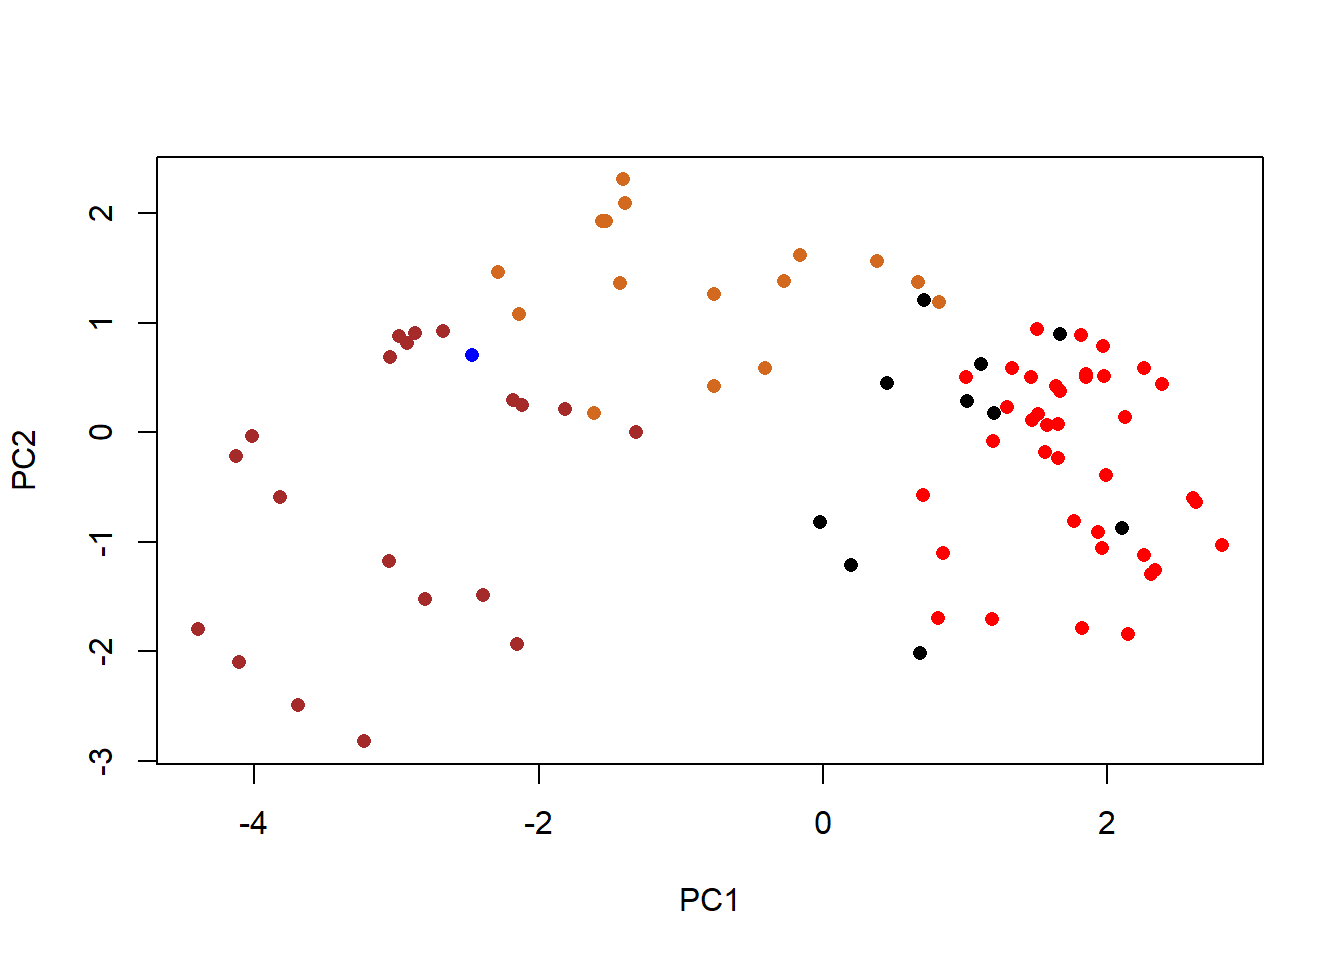
\includegraphics{Halloween-Candy-Mini-Project_files/figure-latex/unnamed-chunk-33-1.pdf}
how do the original variables cols contribute to the new pca. PC1:

\begin{Shaded}
\begin{Highlighting}[]
\NormalTok{loadings }\OtherTok{\textless{}{-}} \FunctionTok{cbind}\NormalTok{(candy, pca}\SpecialCharTok{$}\NormalTok{x[,}\DecValTok{1}\SpecialCharTok{:}\DecValTok{3}\NormalTok{])}
\end{Highlighting}
\end{Shaded}

\begin{Shaded}
\begin{Highlighting}[]
\NormalTok{p }\OtherTok{\textless{}{-}} \FunctionTok{ggplot}\NormalTok{(loadings) }\SpecialCharTok{+}
  \FunctionTok{aes}\NormalTok{(}\AttributeTok{x=}\NormalTok{ PC1, }\AttributeTok{y=}\NormalTok{ PC2, }
      \AttributeTok{text=}\FunctionTok{rownames}\NormalTok{(loadings), }\AttributeTok{fill =}\NormalTok{ PC1, }\AttributeTok{size=}\NormalTok{ winpercent}\SpecialCharTok{/}\DecValTok{100}\NormalTok{) }\SpecialCharTok{+}
  \FunctionTok{geom\_point}\NormalTok{(}\AttributeTok{col=}\NormalTok{mycols)}
  
\NormalTok{  p}
\end{Highlighting}
\end{Shaded}

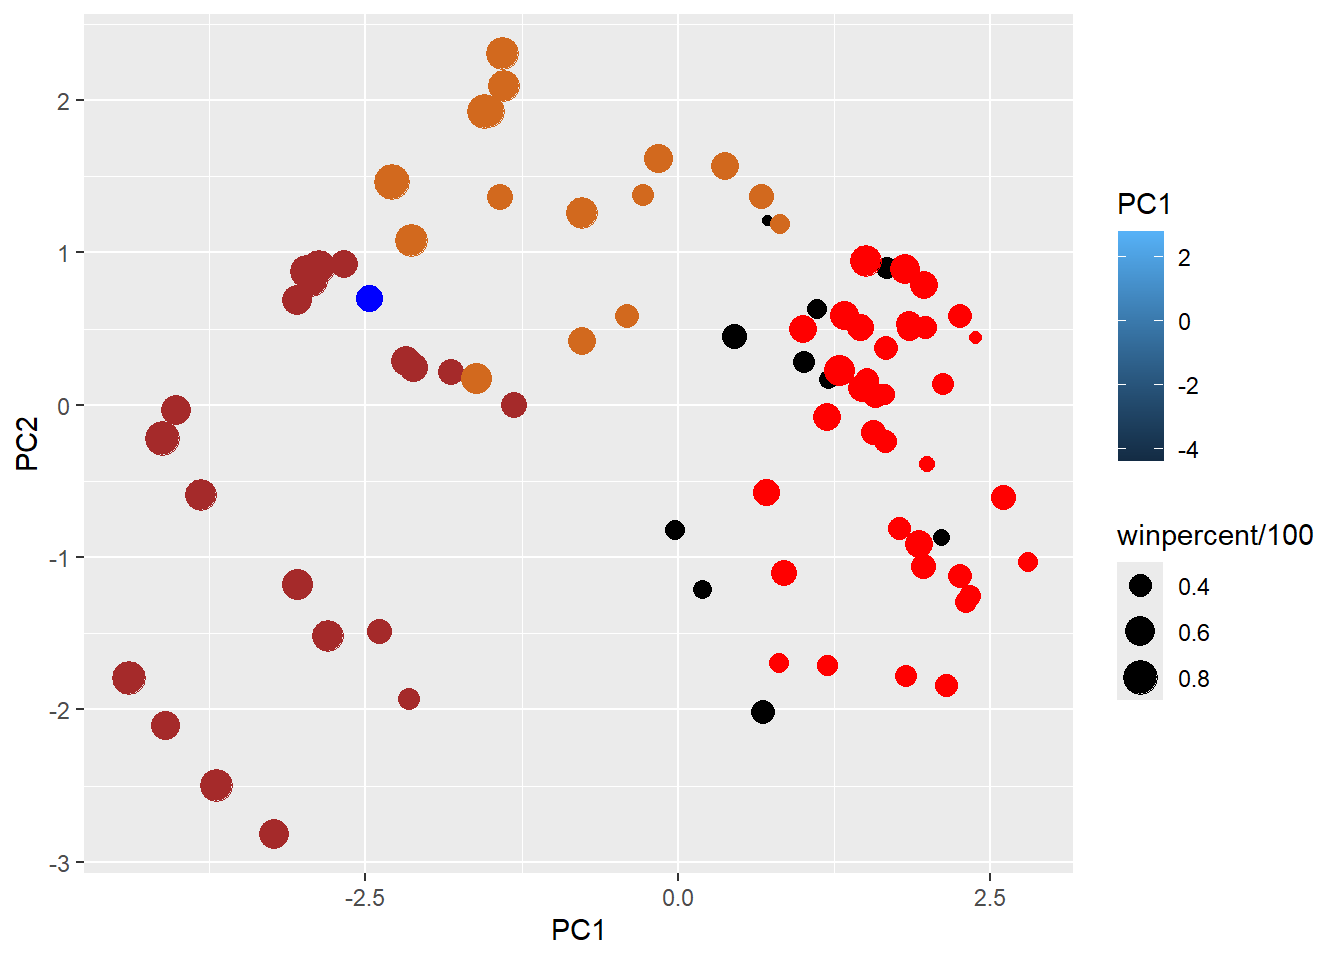
\includegraphics{Halloween-Candy-Mini-Project_files/figure-latex/unnamed-chunk-35-1.pdf}

\begin{Shaded}
\begin{Highlighting}[]
\CommentTok{\#install.packages("ggrepel")}
\FunctionTok{library}\NormalTok{(ggrepel)}

\NormalTok{q }\OtherTok{\textless{}{-}} \FunctionTok{ggplot}\NormalTok{(loadings) }\SpecialCharTok{+}
  \FunctionTok{aes}\NormalTok{(}\AttributeTok{x =}\NormalTok{ PC1, }\AttributeTok{y =}\NormalTok{ PC2, }\AttributeTok{text =} \FunctionTok{rownames}\NormalTok{(loadings), }\AttributeTok{fill =}\NormalTok{ PC1, }\AttributeTok{size =}\NormalTok{ winpercent }\SpecialCharTok{/} \DecValTok{100}\NormalTok{) }\SpecialCharTok{+}
  \FunctionTok{geom\_point}\NormalTok{(}\AttributeTok{col=}\NormalTok{mycols) }\SpecialCharTok{+}
  \FunctionTok{geom\_text\_repel}\NormalTok{(}\FunctionTok{aes}\NormalTok{(}\AttributeTok{label =} \FunctionTok{rownames}\NormalTok{(loadings)), }\AttributeTok{size =} \FloatTok{3.3}\NormalTok{, }\AttributeTok{col =}\NormalTok{ mycols, }\AttributeTok{max.overlaps =} \DecValTok{7}\NormalTok{) }\SpecialCharTok{+} 
  \FunctionTok{theme}\NormalTok{(}\AttributeTok{legend.position =} \StringTok{"none"}\NormalTok{) }\SpecialCharTok{+}
  \FunctionTok{labs}\NormalTok{(}\AttributeTok{title =} \StringTok{"Halloween Candy PCA Space"}\NormalTok{, }\AttributeTok{subtitle =} \StringTok{"Colored by type: chocolate bar (dark brown), chocolate other (light brown), fruity (red), other (black)"}\NormalTok{,}
    \AttributeTok{caption =} \StringTok{"Data from 538"}\NormalTok{)}
\NormalTok{q}
\end{Highlighting}
\end{Shaded}

\begin{verbatim}
## Warning: ggrepel: 44 unlabeled data points (too many overlaps). Consider
## increasing max.overlaps
\end{verbatim}

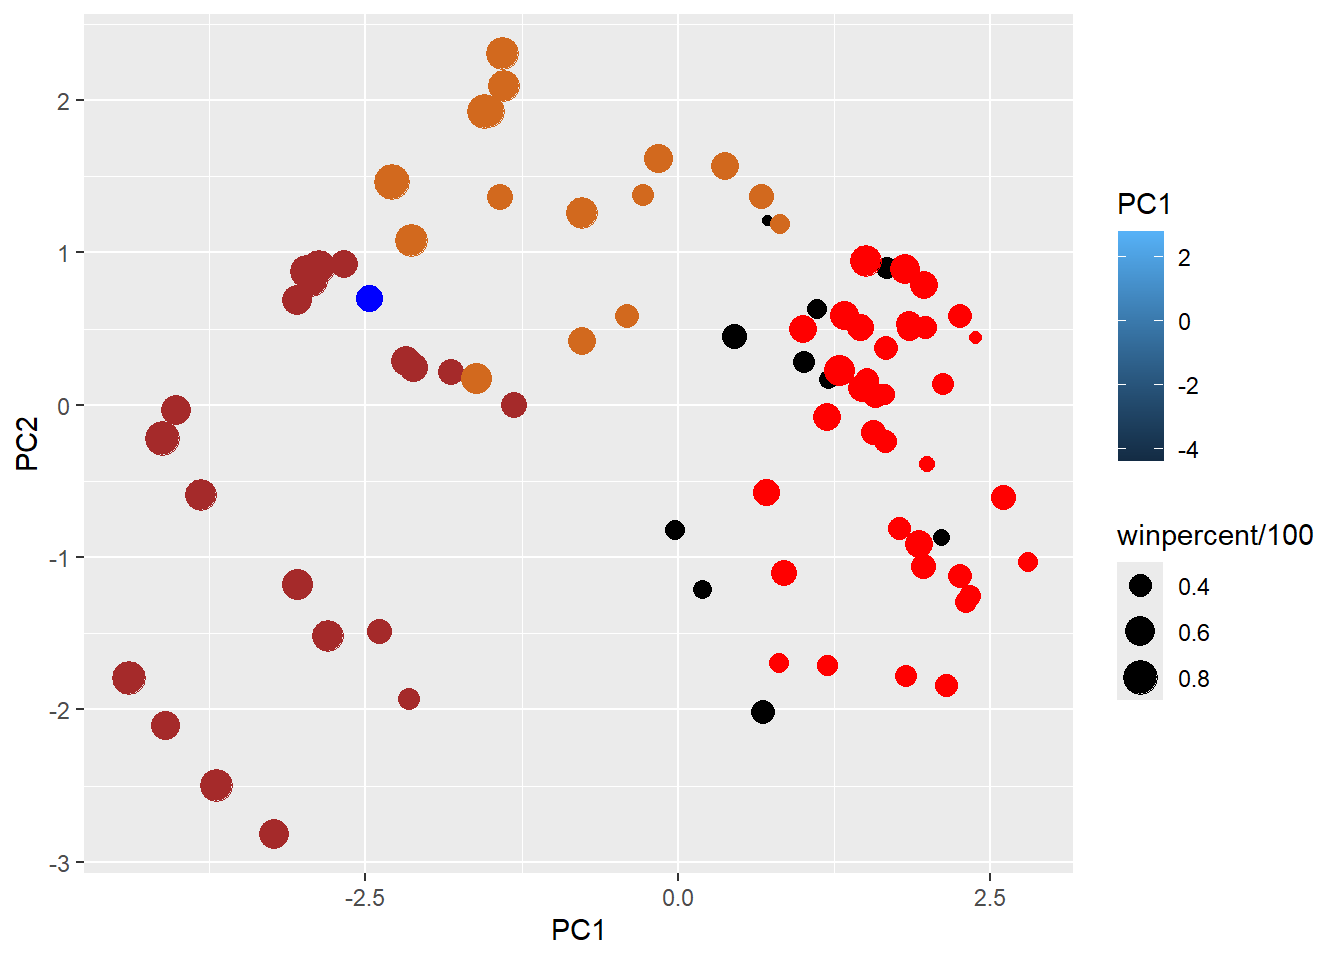
\includegraphics{Halloween-Candy-Mini-Project_files/figure-latex/unnamed-chunk-36-1.pdf}

\begin{Shaded}
\begin{Highlighting}[]
\CommentTok{\#install.packages("plotly")}
\CommentTok{\#library(plotly)}

\CommentTok{\#ggplotly(q)}
\end{Highlighting}
\end{Shaded}

\begin{Shaded}
\begin{Highlighting}[]
\FunctionTok{par}\NormalTok{(}\AttributeTok{mar=}\FunctionTok{c}\NormalTok{(}\DecValTok{8}\NormalTok{,}\DecValTok{4}\NormalTok{,}\DecValTok{2}\NormalTok{,}\DecValTok{2}\NormalTok{))}
\FunctionTok{barplot}\NormalTok{(pca}\SpecialCharTok{$}\NormalTok{rotation[,}\DecValTok{1}\NormalTok{], }\AttributeTok{las=}\DecValTok{2}\NormalTok{, }\AttributeTok{ylab=}\StringTok{"PC1 Contribution"}\NormalTok{)}
\end{Highlighting}
\end{Shaded}

\includegraphics{Halloween-Candy-Mini-Project_files/figure-latex/unnamed-chunk-38-1.pdf}

\begin{quote}
Q24. What original variables are picked up strongly by PC1 in the
positive direction? Do these make sense to you?No,I think it should be
reveresed
\end{quote}

\end{document}
